%% Classe du document
\documentclass[a4paper,10pt]{article}

%% Francisation
\usepackage[francais]{babel} % Indique que l'on utilise le francais
\usepackage[T1]{fontenc}
\usepackage[utf8]{inputenc} % Indique que l'on utilise tout le clavier
%\usepackage[latin1]{inputenc}

%% Réglages généraux
\usepackage[top=3cm, bottom=3cm, left=3cm, right=3cm]{geometry} % Taille de la feuille
\usepackage{lastpage}

%% Package pour le texte
\usepackage{soul} % Souligner
\usepackage{color} % Utilisation de couleurs
\usepackage{hyperref} % Créer des liens et des signets
\usepackage{eurosym}% Pour le symbole euro
\usepackage{fancyhdr}% Entête et pied de page

%% Package pour les tableaux
\usepackage{multirow} % Colonnes multiples
\usepackage{cellspace}
\usepackage{array}

%% Package pour les dessins
\usepackage{pstricks}
\usepackage{graphicx} % Importer des images
\usepackage{pdftricks} % Pour utiliser avec pdfTex
\usepackage{pst-pdf} % Pour utiliser avec pdfTex
\usepackage{pst-node} % Pose de noeuds
\usepackage{subfig}
\usepackage{float}

%% Package pour les maths
\usepackage{amsmath} % Commandes essentielles
\usepackage{amssymb} % Principaux symboles

%% Package pour le code
\usepackage{listings} % Utilisation de la couleur syntaxique des langages
\usepackage{url}


\usepackage[babel=true]{csquotes} % Permet les quotations (guillemets)
\usepackage{tocvsec2}
\usepackage{amsthm}
\usepackage{amsfonts}

\usepackage{tikz}
\usepackage{pdfpages}

\usetikzlibrary{shapes} % A revoir

%--------------------- Autres définitions ---------------------%

% Propriété des liens
\hypersetup{
colorlinks = true, % Colorise les liens
urlcolor = blue, % Couleur des hyperliens
linkcolor = black, % Couleur des liens internes
}

\definecolor{grey}{rgb}{0.95,0.95,0.95}

% Language Definitions for Turtle
%TODO: a revoir avec les couleur de gedit
\definecolor{olivegreen}{rgb}{0.2,0.8,0.5}
\definecolor{grey2}{rgb}{0.5,0.5,0.5}
\lstdefinelanguage{ttl}{
sensitive=true,
morecomment=[s][\color{grey2}]{@}{:},
morecomment=[l][\color{olivegreen}]{\#},
morecomment=[s][\color{red}]{<}{/>},
morestring=[s][\color{olivegreen}]{<http://w}{\#>},
morestring=[b][\color{blue}]{\"},
}

\lstset{%language = sql,
basicstyle =\footnotesize,
%numbers = left,
numberstyle=\normalsize,
numbersep=10pt,
framexleftmargin=5mm,
frame=lines,
tabsize=4}

%Definition de la commande pour retirer l'espace devant les ':'
\makeatletter
\@ifpackageloaded{babel}%
        {\newcommand{\nospace}[1]{{\NoAutoSpaceBeforeFDP{}#1}}}%  % !! double {{}} pour cantonner l'effet à l'argument #1 !!
        {\newcommand{\nospace}[1]{#1}}
\makeatother

\setcounter{tocdepth}{3}
%\maxsecnumdepth{subsubsection} % Dernière section numérotée

\newcommand{\paperPrototyping}{\emph{paper prototyping}}

% Corps du document :
\begin{document}

% Définition des entêtes et pieds de page
\fancyhead[LE,CE,RE,LO,CO,RO]{}
\fancyfoot[LE,CE,RE,LO,CO,RO]{}
\fancyhead[LO, LE]{Programmation par contraintes}
\fancyhead[RO,RE]{2012/2013}
\fancyfoot[LO,LE]{Université de \scshape{Nantes}}
\fancyfoot[RO,RE]{Page \thepage \ sur \pageref{LastPage}}
\renewcommand{\headrulewidth}{0.4pt}
\renewcommand{\footrulewidth}{0.4pt}

%\maketitle
\begin{titlepage}

\vspace*{\fill}~
\begin{center}
{\large \textsc{Rapport de Projet}} \\
\textsc{Tabu Search} \\
\vspace{0.5cm}
COUTABLE Guillaume, RULLIER Noémie \\
\today
\end{center}
\vspace*{\fill}

\vspace{\stretch{1}}
\begin{center}
\noindent 

\includegraphics[height=2.5cm]{Images/universite.png}
\end{center}
\pagebreak
\end{titlepage}

\newpage
\tableofcontents  

% Introduction
\newpage
\pagestyle{fancy}

%%%%%%%%%%%%%%%%%%%%%%%%%%%%%%%%%%%%%%%%%%%%%%%%%%%%%%%%%%%%%%%%%%%%%%%%%%%%%
%%%%%%%%%%  Introduction générale
%%%%%%%%%%%%%%%%%%%%%%%%%%%%%%%%%%%%%%%%%%%%%%%%%%%%%%%%%%%%%%%%%%%%%%%%%%%%%
\section{Introduction}
L'objectif de ce TP fut de comprendre et d'implémenter l'algorithme TabuSearch en JaCoP.

%%%%%%%%%%%%%%%%%%%%%%%%%%%%%%%%%%%%%%%%%%%%%%%%%%%%%%%%%%%%%%%%%%%%%%%%%%%%%
%%%%%%%%%% TS
%%%%%%%%%%%%%%%%%%%%%%%%%%%%%%%%%%%%%%%%%%%%%%%%%%%%%%%%%%%%%%%%%%%%%%%%%%%%%
\section{Présentation du TabuSearch}
Tabu search est une heuristique de la méthode de recherche locale. Elle consiste dans un premier temps à générer affectation totale des variables. Elle va ensuite effectuer le mouvement qui a un coût le moins important. Tabu search permet d'ajouter une contrainte, en effet on marque les $p$ derniers mouvements effectués qui seront interdits. On répète cette dernière opération jusqu'à ce que le coût soit égal à 0 ou jusqu'à ce que le nombre maximum d'essai soit atteint.

\section{N-Queens avec TabuSearch et CompleteSearch comparaison}

Ces comparaisons ont été effectuées pour différentes valeurs de n (représentant le nombre de reine). L'algorithme \emph{CompleteSearch} a été exécuté avec l'heuristique \emph{Depth First Search}.

Pour chaque valeur n, l'algorithme a été lancé 100 fois. Le temps présenté est la moyenne de ces 100 résultats. Le \emph{Number of errors} représente le nombre de fois où l'algorithme n'a pas trouvé de solution; dans le cas du TabuSearch ce cas peut arriver lorsque le nombre maximum de tour de boucles est atteint sans qu'aucune solution soit trouvée. \newline

\noindent
\begin{tabular}{|c|c|c|}
\hline
\multicolumn{3}{|c|}{CompleteSearch}\\
\hline
n & Number errors & Execution Time (ms) \\
\hline
1 & 0 & 0.2\\
\hline
2 & 100 & 0.45\\
\hline
3 & 100 & 0.77\\
\hline
4 & 0 & 1.6\\
\hline
5 & 0 & 2.77\\
\hline
10 & 0 & 60.22\\
\hline
13 & 0 & 7717.57\\
\hline
>16 & \multicolumn{2}{c|}{No result (OutOfMemory)}\\
\hline
\end{tabular}
\begin{tabular}{|c|c|c|}
\hline
\multicolumn{3}{|c|}{TabuSearch}\\
\hline
n & Number errors & Execution Time (ms) \\
\hline
1 & 0 & 0.13\\
\hline
2 & 100 & 0.83\\
\hline
3 & 100 & 1.01\\
\hline
4 & 0 & 0.47\\
\hline
5 & 0 & 0.56\\
\hline
10 & 36 & 2.98\\
\hline
13 & 31 & 10.52\\
\hline
20 & 35 & 20.55\\
\hline
30 & 47 & 102.39\\
\hline
50 & 45 & 692.37\\
\hline
75 & 31 & 3312.75 \\
\hline
100 & 23 & 10776.28 \\
\hline
\end{tabular}

\begin{figure}[H]
    \center
    \subfloat[Execution time]{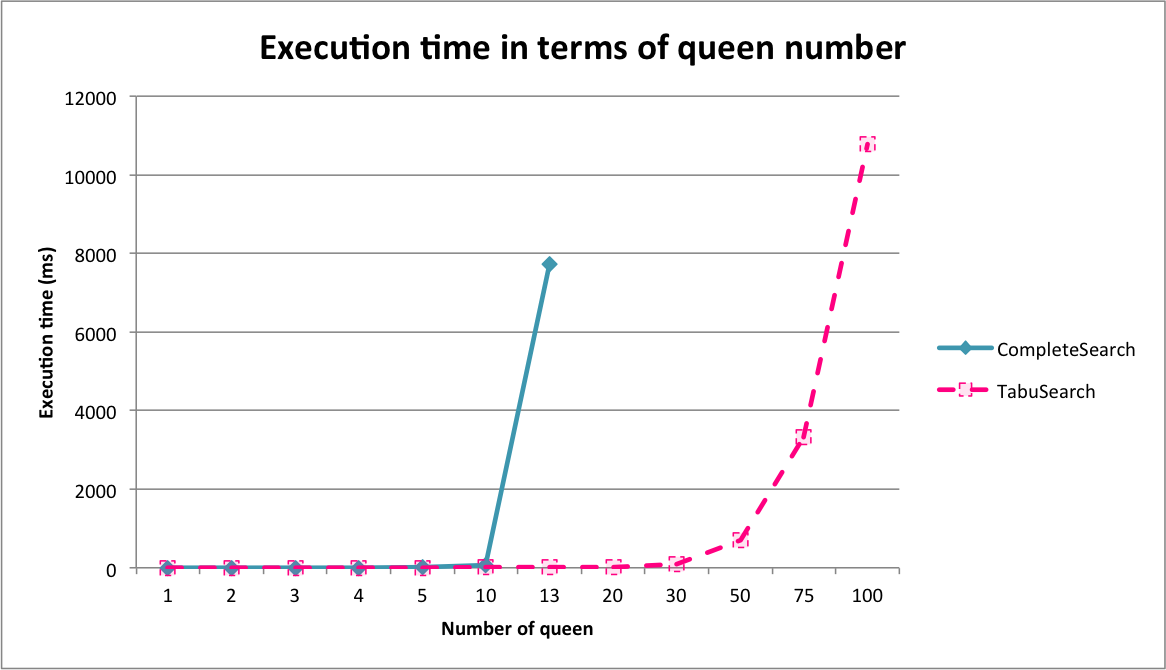
\includegraphics[width=7.3cm]{Images/TS_ExecTime.png}} \quad
    \subfloat[Number of errors]{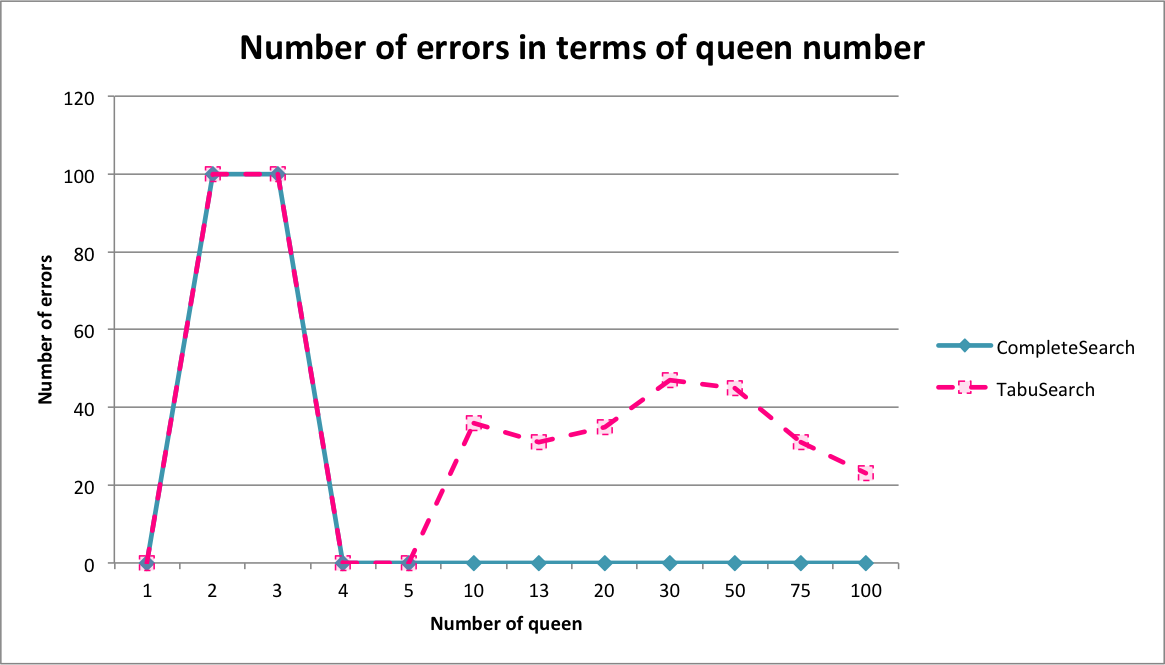
\includegraphics[width=7.3cm]{Images/TS_NumberErrors.png}}
    \caption{Graph of comparaison between CompleteSearch and TabuSearch}
\end{figure}
On peut voir que pour $n$ égal à $2$ et $3$, aucune solution n'est jamais trouvée. En effet, ce problème n'est pas consistent.

On peut de plus constater que pour $n>13$, l'algorithme \emph{CompleteSearch} ne permet pas de résoudre le problème. La façon dont celui-ci recherche les solutions engendre une exception \emph{OutOfMemory}.

On peut remarquer que plus le nombre de $n$ de reines augmente plus le temps d'exécution augmente (de façon exponentielle). Cette remarque est valable pour les deux algorithmes testés.

On peut cependant noter que le \emph{TabuSearch} permet de trouver la solution pour un plus grand nombre de reines. Si l'on compare les deux algorithmes, pour le même nombre de reines donnés \emph{TabuSearch} est plus rapide.

La dernière remarque que l'on peut faire, concerne le nombre d'erreurs. Ceux-ci ne sont pas réguliers pour le \emph{TabuSearch} car en effet tout dépend de la première solution générée aléatoirement, du nombre d'itération maximum donnés (ici nous avons choisi 100) et de la taille de la liste des éléments tabous. 

\section{Ajout des conditions d'aspirations}
Les conditions d'aspirations permettent d'autoriser un élément tabou s'il améliore la meilleure solution.

\section{TabuSearch algorithme avec procédure de redémarrage}

\end{document}

